 
\section{Cosmic Rays}

%% Introduction of cosmic ray field
The humankind has been continuously driven by the curiosity to explore the unknown world. Up to today the highest particle energy that can be achieved through man-made particle accelerators is at the few TeV scale. To study the beyond, our universe itself serves as a tool. Universe is the ultimate laboratory for particle physics.  \par 

%% Cosmic ray spectrum (knee, ankle, limit)
The spectrum of cosmic rays covers an incredibly wide range in intensity and energy. The measured cosmic ray flux is seen at Earth varying about 31 orders of magnitude, which corresponds to the scale of the visible Universe compared to the human hair diameter. The measured energy of cosmic rays can go up to the ZeV level ($10^{21}$ eV), such an unprecedented energy can not be currently generated by man-made facilities. The large dynamic range can be seen in figure \ref{CosmicRayFluxVersusParticleEnergy}. As shown in this figure, the cosmic ray flux follows a power law: 

\begin{equation}
\Phi(E)\propto E^{-\gamma}
\end{equation}

where $\Phi$ is the flux, $E$ is the energy and $\gamma$ is the spectral index.

The spectral index of the cosmic ray is around 2.7. Below $10^{10}$ eV (10 GeV) the flux is lower than the power law extrapolation because low energy particles can be deflected by the solar magnetic field and not reach around the Earth. From around $3 \times 10^{15}$ (3 PeV) to $4 \times 10^{18}$ eV (4 EeV), the spectrum index steeps to around 3.1, which is called "knee". Above 4 EeV the spectrum index backs to around 2.7, the transition period is called "ankle". In addition, although the theoretical upper limit on the energy of cosmic ray protons, the  Greisen–Zatsepin–Kuzmin (GZK) limit, is equal to $5 \times 10^{19}$ eV (50 EeV) \cite{GZKPaper1, GZKPaper2}, there are experiments, which appear to have detected cosmic rays with energies higher than this limit \cite{OMGParticle1, OMGParticle2}. This fact poses an unsolved puzzle that needs to be investigated. These features and observations are important to understand the sources of cosmic rays and their propagation.  \par

%% Cosmic ray Components
% Space Experiment AMS-02
Earth is constantly bombarded by subatomic particles. Due to the Earth’s atmosphere, the ground-based cosmic rays experiments can only measure cascades of cosmic rays. To measure the cosmic rays directly, detectors have to be placed above the atmosphere. The AMS-02 experiment is conducted on the ISS, which maintains an orbit with an average altitude of 417 km, therefore it can precisely measure the cosmic rays avoiding their interactions with the atmosphere. \par

\begin{figure}[H]    
\subfigure[] { \label{CosmicRayFluxVersusParticleEnergy}    
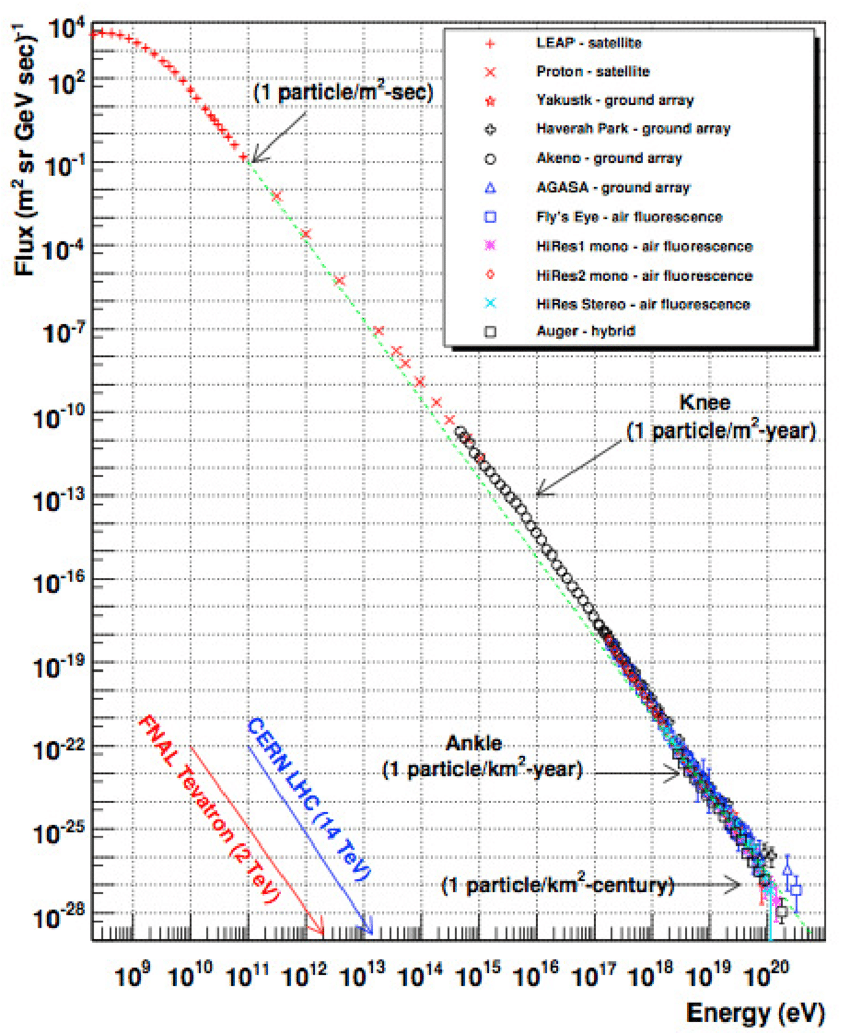
\includegraphics[width=0.45\columnwidth, height=0.4\textheight]{Figures/chapter2/Cosmicrays/CosmicRayFluxVersusParticleEnergy.png} 
}    
\subfigure[] { \label{CosmicRaysComponentsFlux}    
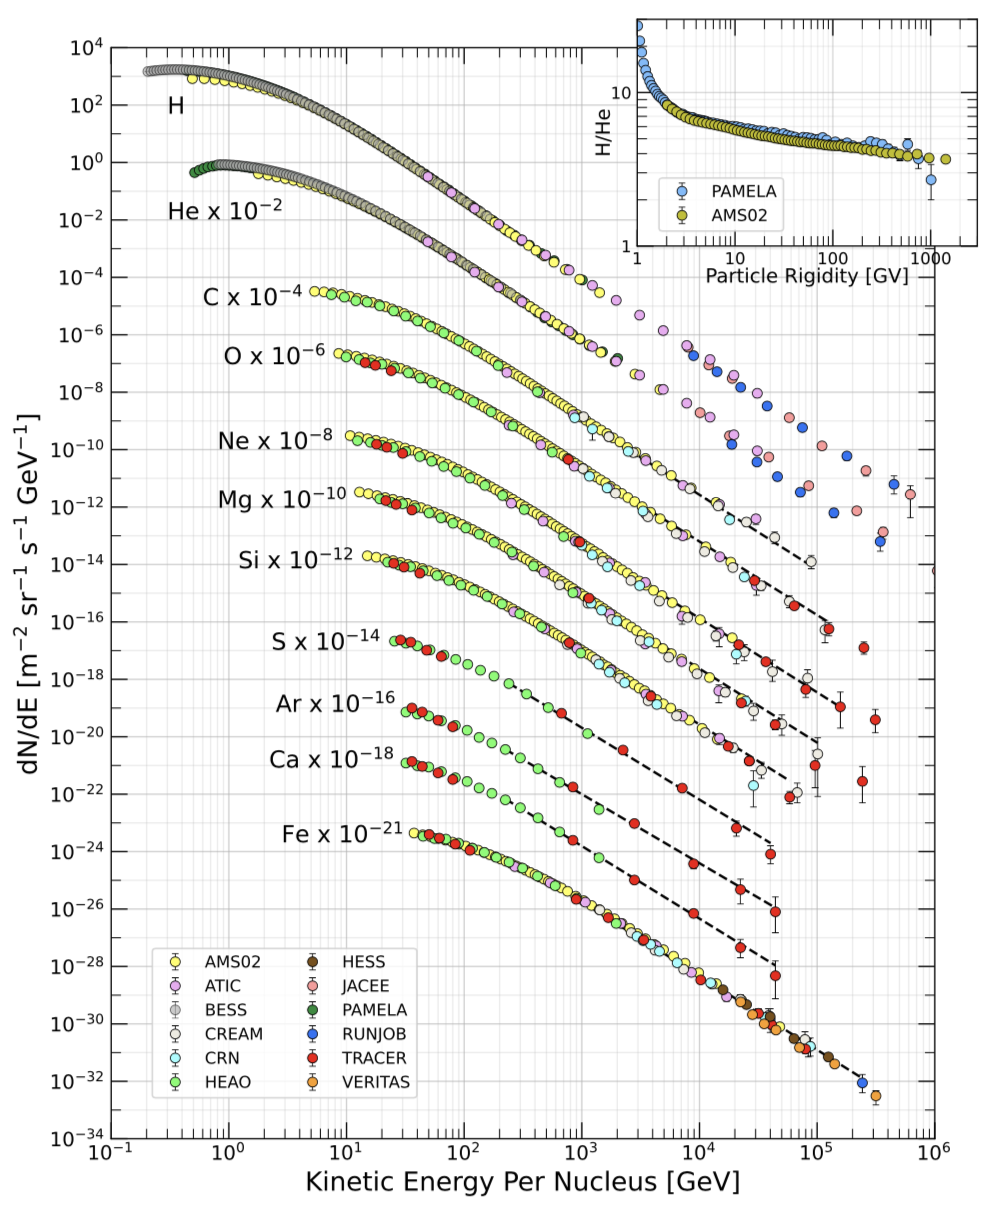
\includegraphics[width=0.45\columnwidth, height=0.4\textheight]{Figures/chapter2/Cosmicrays/CosmicRaysComponentsFlux.png}    
}    
\caption[Cosmic ray spectrum and components]{a) Cosmic ray spectrum has a wide range in flux and energy \cite{CosmicRaysKneeAndAnkle}, the knee is at around 1 PeV and the ankle is at 4 EeV. b) The fluxes of different components of cosmic rays follow a universal power law trend \cite{PDG2020}. }
\end{figure}

% Primary and secondary cosmic rays
There are two kinds of cosmic rays: primary and secondary. Primary cosmic rays are produced in astrophysical sources, while secondary cosmic rays are produced from the interactions between the primary cosmic rays and the interstellar medium. Primary cosmic rays mainly comprise protons, electrons, He, C, O, Ne, Mg, Si, Fe and others. Secondary cosmic rays consist of mainly positrons, antiprotons, Li, Be, B, F, and others. The precise measurement of cosmic rays can provide information about the astrophysical sources and also the propagation processes as well. \par

%都有:N, Na, Al,
\begin{comment}  %% AMS publication 
Primary iron cosmic rays are the most abundant heavy nuclei beyond silicon. They are thought to be mostly produced and accelerated in astrophysical sources. Iron interaction cross sections with the interstellar medium (p, He) are significantly larger than those of lighter nuclei (He, C, O, Ne, Mg, and Si). Therefore, iron nuclei interact much more with the interstellar medium during propagation. Precise knowledge of the iron spectrum in the GV–TV rigidity region provides important information on the origin, acceleration, and propagation processes of cosmic rays in the Galaxy [1]. Previously, the precision measurements of the primary cosmic ray He, C, and O fluxes and Ne, Mg, and Si fluxes with the Alpha Magnetic Spectrometer experiment (AMS) have been reported [2,3]. These measurements revealed an identical rigidity dependence of the He, C, and O fluxes above 60 GV and their deviation from a single power law (hardening) above ∼200 GV. The AMS results also revealed unexpected differences in the rigidity dependence of the Ne, Mg, and Si fluxes compared to the He, C, and O fluxes. To date, iron nuclei (Z 1⁄4 26) are the highest charge cosmic rays measured by AMS. The rigidity dependence of the iron flux compared with that of lower-charge primary cosmic rays provides new insights into the origin and propagation of cosmic rays [4,5].

Carbon nuclei in cosmic rays are thought to be mainly produced and accelerated in astrophysical sources, while boron nuclei are entirely produced by the collision of heavier nuclei, such as carbon and oxygen, with nuclei of the interstellar matter. Therefore, the boron to carbon flux ratio (B=C) directly measures the average amount of interstellar material traversed by cosmic rays.
\end{comment}


% all the components follow a power law
Cosmic rays consist of many components. For primary cosmic rays, ~89\% are protons, 10\% are helium nuclei and around 1\% are heavy elements. In figure \ref{CosmicRaysComponentsFlux} the fluxes of different cosmic ray components are shown. A universal power law spectrum is observed in all kinds of cosmic rays, which supports the assumption of a general electro-magnetic acceleration mechanism, though small differences still need to be investigated. With the efforts of different measurements, the fluxes of cosmic ray components have been measured for a large energy range.     \par

\begin{figure}[h] 
\centering
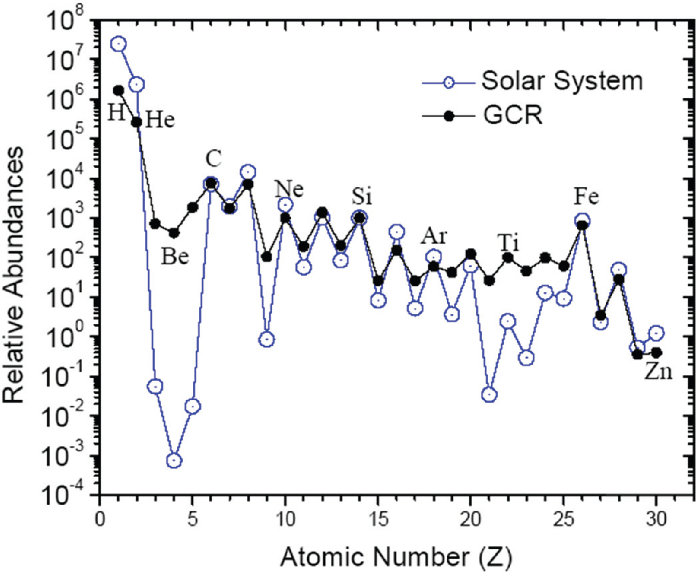
\includegraphics[width=0.9\textwidth, height=0.45\textheight ]{Figures/chapter2/Cosmicrays/Galactic-cosmic-ray-relative-abundances-compared-with-the-Solar-System-ones-The-curves.png}
\caption[Element abundances between the GCR and the solar system]{A good agreement of element abundances between the GCR and the solar system is shown \cite{ElementAbundanceOfCosmicRays_OriginalACE}, except some differences like over-abundance of H and He in solar system, excess of Li, Be, B in GCR and others.}
\label{ElementAbundanceOfCosmicRays}
\end{figure}

% 
In figure \ref{ElementAbundanceOfCosmicRays}, the abundances of the galactic cosmic rays (GCR) arriving near Earth compared to the ones of the solar system are shown. In general, there is good agreement between these two kinds of abundances, the differences illustrate the part of secondary production of cosmic rays. The reduced abundance of the galactic cosmic hydrogen and helium is due to the effects of the solar magnetic field. Due to the spallation and interactions of the cosmic rays, the C, N and O nuclei would break into elements of lower mass, namely Li, Be, and B. This fact explains the higher abundances of Li, Be and B in the GCR.  

%% ground and space measurement(待定)




